\subsection{Good Suffix Regel}
\vspace*{-0.5\baselineskip}\begin{itemize}[itemsep=-1pt]
	\item Mismatch bei $j=m-x$ mit $P[x,\dots,l]$ ist der am weitesten rechts liegende Teil-String von $P[1,\dots,m-1]$, der mit $P[j+1,\dots,m]$ übereinstimmend
	\item $s$ kann um $m-l$ erhöht werden
	\item die Funktion $s_P(j)$ ist die Länge des größten Präfixes von $P$, sodass eine der folgenden Eigenschaften gilt:
		\begin{enumerate}
			\item $P[j+1,\dots,m]$ ist ein Suffix von $P[1,\dots,s_P(j)]$ und $P[j] \neq P[s_P(j)-m+j]$\\\up
				\usetikzlibrary{positioning,patterns}

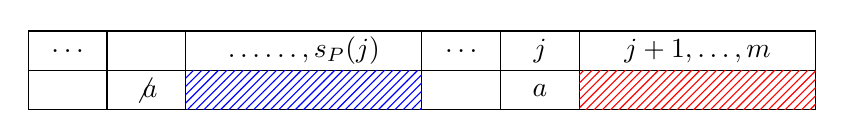
\begin{tikzpicture}[]

\draw(0,0)rectangle(10,1);
\draw(0,0)rectangle(10,0.5);

\foreach \x in {1,2,5,6,7}
	\draw(0,0)rectangle(\x,1);

\node at (0.5,.75) {$\dots$};
\node at (3.5,.75) {$\dots\dots,s_P(j)$};
\node at (5.5,.75) {$\dots$};
\node at (6.5,.75) {$j$};
\node at (8.5,.75) {$j+1,\dots,m$};

\node at (1.5,0.25) {$\not{a}$};
\node[pattern=north east lines,minimum height=0.5cm,minimum width=3cm,pattern color=blue] at (3.5,0.25) {};
\node at (6.5,0.25) {$a$};
\node[pattern=north east lines,minimum height=0.5cm,minimum width=3cm,pattern color=red] at (8.5,0.25) {};

\end{tikzpicture}
			\item[] oder
			\item $P[1,\dots,s_P(j)]$ ist ein Suffix von $P[j+1,\dots,m]$\\\up
				\usetikzlibrary{positioning,patterns}

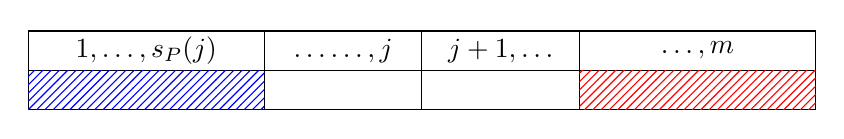
\begin{tikzpicture}[]

\draw(0,0)rectangle(10,1);
\draw(0,0)rectangle(10,0.5);

\foreach \x in {3,5,7}
	\draw(0,0)rectangle(\x,1);

\node at (1.5,.75) {$1,\dots,s_P(j)$};
\node at (4,.75) {$\dots\dots,j$};
\node at (6,.75) {$j+1,\dots$};
\node at (8.5,.75) {$\dots,m$};

\node[pattern=north east lines,minimum height=0.5cm,minimum width=3cm,pattern color=blue] at (1.5,0.25) {};
\node[pattern=north east lines,minimum height=0.5cm,minimum width=3cm,pattern color=red] at (8.5,0.25) {};

\end{tikzpicture}
			\item[]\begin{description}
				\item[Hinweis:] die roten und blauen Flächen können sich in den einzelnen Fällen überschneiden
				\end{description} 
		\end{enumerate}
	\item wenn das am weitesten rechts liegende Mismatch bei $j$ in $P$ auftaucht, kann die Verschiebung $s$ um $m-s_P(j)$ erhöht werden (\algo{Algorithmus von Boyer und Moore (mit \textcolor{red}{Galil-Erweiterung})}{arg2})
	\item ist auch gut für große Alphabete
	\item \begin{description}
		\item[Laufzeit:]\ \\\up
			\begin{itemize}
				\item wenn nur die Good-Suffix-Regel angewendet wird, werden im schlechtesten Fall $3n-o(n)$ Vergleiche zwischen Zeichen ausgeführt
				\item Laufzeit ist nur dann sublinear, wenn die Bad-Character-Regel auch angewendet wird
				\item allgemein: $\Theta(m(n-m+1))$ (z.B. $T=a^n,P=a^m$)
				\item mit der Erweiterung von Galil: linear
				\item die Modifikation verhindert das vergleichen von schon bekannten Teil-Zeichenketten (wobei $s_P(j)=\pi(m)$)
			\end{itemize}
	\end{description}
\end{itemize}